\chapter{Theory}
This experiment illustrates the different modes of vibration of a one-dimensional lattice by means of a mechanical model.
The objective of the experiment is to determine the dispersion relation $\omega(k)$ of this model and use it to conclude the mechanical properties of the setup.

\section{Group-/Phase velocity}
A wave can be characterized by its angular frequency $\omega$ and wave number $k$.
With these quantities, we can define its \textbf{phase velocity}
\begin{equation*}
	v_\text{ph}=\frac{\omega}{k},
\end{equation*}
the velocity at which same phases of a wave propagate in space.
In the same manner, a \textbf{group velocity}
\begin{equation*}
	v_\text{gr}=\frac{\d\omega}{\d k},
\end{equation*}
the speed at which a wave's modulation - hence information - travels through space is defined.
In a given medium, the frequency is some function $\omega(k)$, so in general, the group- and phase velocities depend on the medium and are equal only if the \textbf{refractive index} $n=\frac{c}{v_\text{ph}}$ is constant.

\section{The First Brillouin Zone}
The first Brillouin zone is the Wigner-Seitz-cell of the reciprocal lattice.
For a primitive cubic crystal system with lattice parameter $a$, the first Brillouin zone extends across the interval $k\in [-\frac{\pi}{a}, \frac{\pi}{a}]$ in reciprocal space.

Consider a linear chain of coupled atoms.
As a consequence of the discrete nature of this system, the number of physically distinguishable vibration modes is finite, where $\lambda_\text{min}=2a$ and $\lambda_\text{max}=2L$ ($L$ denotes the chain's length) are the minimum and maximum wavelengths.
Defining a \textbf{mode number} $n=\frac{2L}{\lambda_n}$, it follows that the maximal number of possible modes is
\begin{equation*}
	n_\text{max}=\frac{2L}{\lambda_\text{min}}=\frac{L}{a},
\end{equation*}
which is equal to the number of atoms in the chain.

In the same fashion, the maximum wave number is
\begin{equation*}
	k_\text{max}=\frac{2\pi}{\lambda_\text{min}}=\frac{\pi}{a},
\end{equation*}
which is equal to the boundaries of the first Brillouin zone of a primitive cubic lattice.
Therefore, the first Brillouin zone already contains every wave number $k$ that is relevant to the description of distiguishable vibration modes.

\section{Model}
A series of weights connected by springs is used as a model.
The weights ride on a linear air bearing and can move freely in one direction.
Several approximations are made in order to make this model possible:
\begin{itemize}
	\item The force between nodes is approximated by a harmonic potential,
	\item weights can only interact with immediate neighbors and
	\item any effects arising from quantum mechanics are disregarded.
\end{itemize}

\section{Identical Weights}\label{sec:single_theory}
\subsection{Theoretical Background}
\begin{figure}[tbp]
	\centering
	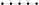
\includegraphics[width=0.6\textwidth]{./img/chain_single.pdf}
	\caption[Chain of Identical Weights]{\textbf{Linear chain of identical weights}}
	\label{fig:chain_single}
\end{figure}
\begin{figure}[tbp]
	\centering
	\includegraphics[width=0.6\textwidth]{./data/plots/dispersion_single.pdf}
	\caption[Dispersion Relation of Chain With Identical Weights]{\textbf{Dispersion relation of a chain with identical weights} Every possible frequency occurs within the range from 0 to $\frac{\pi}{a}$, which means any wave number outside this range is indistinguishable from another oscillation within it.}
	\label{fig:dispersion_single}
\end{figure}
A chain of identical weights with mass $m$, linked by springs with stiffness $D$ and length $a$ is considered (as seen in \autoref{fig:chain_single}).
The newtonian equation of motion for the displacement $x_j$ of the $j$-th element of the chain is
\begin{equation*}
	m \ddot x_j = D \cdot \left(x_{j - 1} + x_{j + 1} - 2 x_j \right).
\end{equation*}
The equation can be solved by the ansatz
\begin{equation*}
	x_j(t) = A \exp\left[\text{i} \left(k a j - \omega t\right)\right],
\end{equation*}
which yields the dispersion relation
\begin{equation}
	\omega(k) = \sqrt{\frac{4D}{m}}\abs{\sin\left(\frac{ka}{2}\right)},
\end{equation}
which is depicted in \autoref{fig:dispersion_single}.

For small $k$, it holds that $\sin(x)\approx x$.
This approximation can be employed for the dispersion relation, so we get
\begin{equation*}
	\omega(k)\approx \sqrt{\frac{Da^2}{m}}\abs{k}.
\end{equation*}
From the above equation, it follows that the phase- and group velocity are identical
\begin{equation}\label{eq:sound_single}
	v_\text{ph} = v_\text{g}\approx \sqrt{\frac{Da^2}{m}}.
\end{equation}

\subsection{Experimental Model}\label{subsec:exp_mod_single}
The model used in this experiment consists of 12 identical weights and 13 identical springs with $L=12\cdot a$.
Hence, the possible modes are
\begin{equation*}
	k_n = \frac{n\pi}{L} = \frac{n\pi}{12a}\quad n\in[1, 12].
\end{equation*}

\section{Alternating Weights} \label{sec:alt_theory}
\subsection{Theoretical Background}
\begin{figure}[tbp]
	\centering
	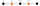
\includegraphics[width=0.6\textwidth]{./img/chain_alternating.pdf}
	\caption[Chain of Alternating Weights]{\textbf{Linear chain of alternating weights}}
	\label{fig:chain_alternating}
\end{figure}
\begin{figure}[tbp]
	\centering
	\includegraphics[width=0.6\textwidth]{./data/plots/dispersion_alternating.pdf}
	\caption[Dispersion Relation of Chain With Alternating Weights]{\textbf{Dispersion relation of a chain with alternating weights} Between the photonic and acoustic branches of the dispersion curve, a \textbf{band gap} is visible (colored in red). Waves with frequencies within this gap cannot propagate.}
	\label{fig:dispersion_alternating}
\end{figure}
A chain of weights with alternating masses $m_1$ and $m_2$, linked by identical springs with stiffness $D$ and length $a$ is considered (as seen in \autoref{fig:chain_alternating}).
The index $j$ denotes the $j$-th unit cell, which contains the weights $m_1$ with displacement $u_j$ and $m_2$ with displacement $v_j$.
The newtonian equations of motions are
\begin{gather*}
	m_1 \ddot u_j = D \cdot \left(v_{j - 1} + v_{j} - 2 u_j \right)\\
	m_2 \ddot v_j = D \cdot \left(u_{j} + u_{j + 1} - 2 v_j \right).
\end{gather*}
The equation can be solved by the ansatz
\begin{gather*}
	u_j(t) = U \exp\left[\text{i} \left(2 k a j - \omega t\right)\right]\\
	v_j(t) = V \exp\left[\text{i} \left(k a (2 j + 1) - \omega t\right)\right].
\end{gather*}
This yields the dispersion relation
\begin{equation}
	\omega_\pm^2(k) = \frac{D}{\mu} \pm D\sqrt{\frac{1}{\mu^2} - \frac{4}{m_1 m_2}\sin^2\left(k a\right)},
\end{equation}
with the reduced mass $\mu = \frac{m_1 m_2}{m_1 + m_2}$.

For crystals with at least two different atoms in their primitive cell, the dispersion relation features two types of phonons, namely, acoustic and optical modes.
They correspond to the $\omega_{+}$ and $\omega_{-}$ solutions respectively, which are shown in the dispersion relation \autoref{fig:dispersion_alternating}.
In acoustic modes, all atoms share the same phase, whereas in optical modes, all atoms of each kind are out of phase by \SI{180}{\degree} relative to the other kind.
As a consequence, there is a band gap between optical and acoustic modes.
Phonons with a frequency within this gap cannot propagate in the crystal.

Again, for small $k$, it holds that $\sin(x)\approx x$.
Expanding the root to the first order, it follows that
\begin{align*}
	\omega_{-}(k) &\approx \sqrt{\frac{Da^2}{m_1+m_2}}\abs{k}. \\
	\omega_{+}(k) &\approx \sqrt{2D\mu}.
\end{align*}
Considering the positive solution approximation, it follows that the phase- and group velocity are, again, identical
\begin{equation}\label{eq:sound_alternating}
	v_\text{ph} = v_\text{g}\approx \sqrt{\frac{Da^2}{m_1+m_2}}.
\end{equation}
\subsection{Experimental model}\label{subsec:exp_mod_alternating}
In the setup an additional weight is added to every other slider.
The primitive cell now contains two weights, so $L=\num{6}\cdot a$.
This results in the possible modes
\begin{equation*}
	k_n = \frac{n\pi}{L} = \frac{n\pi}{\num{6}a}\quad n\in[1, 6].
\end{equation*}
